\chapter{Methodology and Implementation}\label{chap:meth_and_impl}

	\paragraph{} 
	Here in this chapter we will discuss the methods applied to extract an explicit model from an \ac{epr} problem specification. And how they are implemented using E's data structures and configurations.

	\paragraph{} 
	\textbf{In order to achieve our goal,} we had to transform the problems' clauses, which are the axioms of the specification and the negated conjectures(if found), to clauses in range restricted form through a simplified form of range restricted transformations. The original range restricted transformations and there simplified version will be discussed in section \ref{sec:c3s1}.  

	\section{Transformations}\label{sec:c3s1}
The methods applied in the project to extract the models follows the transformations discussed in \cite{BMUG06}. A brief on the original transformations will be given in \ref{sub:c3s1s1}.


Moreover, as mentioned before that this project is concerned with a sub-class of \ac{fol} which is \ac{epr} some simplifications to the transformations were made as the removed steps will have no meaning in the context of \ac{epr} problems. Those simplifications will be discussed in \ref{sub:c3s1s2}.

	\subsection{Original transformations}\label{sub:c3s1s1}
	\paragraph{The original procedures} discussed in \cite{BMUG06} generally work for all sub-classes of \ac{fol}. Those procedures should be applied to a given set of axioms in a specific form called implication form, sometimes it is called a sequent as in here ---ref---, which is explained here -- , and here -- to know how to transform to that form. Moreover, those transformations are guranteed to terminate for any given problem set, which is a gain for us since some of the \ac{epr} problems were not terminating in the original configurations of E.  
%TODO :: to add a reference later

	\subsubsection{What are the Transformations}
	
		\paragraph{} 
		\textbf{The Transformations} are series of procedures, mainly about changing the clauses to certain form named range restricted form. Since the transformations deal with clauses in implication form, then we could define \textbf{Clauses in range restricted form} \ul{to be clauses in which all the variables that appear in the succeedent must exist in the anticedent as well}.
	
		\paragraph{} 
		\textbf{An example for a range restricted clause} is found below:
			\begin{lstlisting}[caption=Range Restricted Clause Example,frame=single,mathescape]			
		
		$ \forall X \forall Y  \left( P(X) \wedge Q(Y) \longrightarrow R(X, Y) \right). $				
		
	where the $\textbf{antecedent}$ here is $ P(X) \wedge Q(Y) $;
	whereas the $\textbf{succeedent}$ is $ R(X, Y) $.
 			\end{lstlisting}
		
		
		\paragraph{} 
		\textbf{For a reason} why this range restricted form will help would be ??
%TODO :: add the reason later

	 \subsubsection{How do the transformations work}
	 
		\paragraph{} 
		\textbf{Transformations} add a domain predicate to the specification that will help in finding the Model by saying what are the elements of the domain, or the elements of the universe in other words.\par
		Moreover, There are three types of procedures in the transformations:	
		\begin{itemize}
			\item \textbf{Range restricting transformations}
			 \hfill \\ are the first two transformations, and they are the most important type of them. All the rest were added to enhance and improve the range restricting ones. They are responsible for transforming the input clauses to the range restricted form and enumerating the universe/domain of the problem in a way or another. Only one of the two transformations should applied, since they perform the same functionality but in different ways. The two transformations are:
			 	\begin{itemize}
			 		\item \ac{crr}: it enumerates the Herbrand Universe in a naive simple way. 
			 		\item \ac{rr}: it was introduced to improve the naive implementation of the \ac{crr}. So it only adds elements to the domain only when it is needed.
			 	\end{itemize}
			
			\item \textbf{Shifting transformations}
			 \hfill \\ are the second two transformations. They are optional to be used. They complement one another not replace each other. They were introduced mainly to prevent the non-termination of the transformations and to prevent generating and redundant and unpleasant clauses from the steps in \ac{rr} as well. And the two shifting transformations are:
			 	\begin{itemize}
			 		\item \ac{bs}
			 		\item \ac{pf}
			 	\end{itemize}
			
			\item \textbf{\ac{bl}}
			 \hfill \\ is the last transformation and it is optional as well. And It was introduced to detect periodicity that may occur because of function terms. 
		\end{itemize}
		
		\paragraph{} \textbf{Their order of application} is:
			\begin{enumerate}
				\item One of the two range restricting \ac{crr} or \ac{rr}
				\item The Partial Flattening \ac{pf}
				\item The Basic Shifting \ac{bs}
				\item The Blocking \ac{bl} 
			\end{enumerate}			 
		Where the output of a lower number transformation is the input to the higher one. A Flow Chart that summarizes what was explained will be found in Figure ~\ref{fig:original_transformations_flow}.
		
		\begin{figure}[H]
			\centering
 		 	\scalebox{0.38}
 			{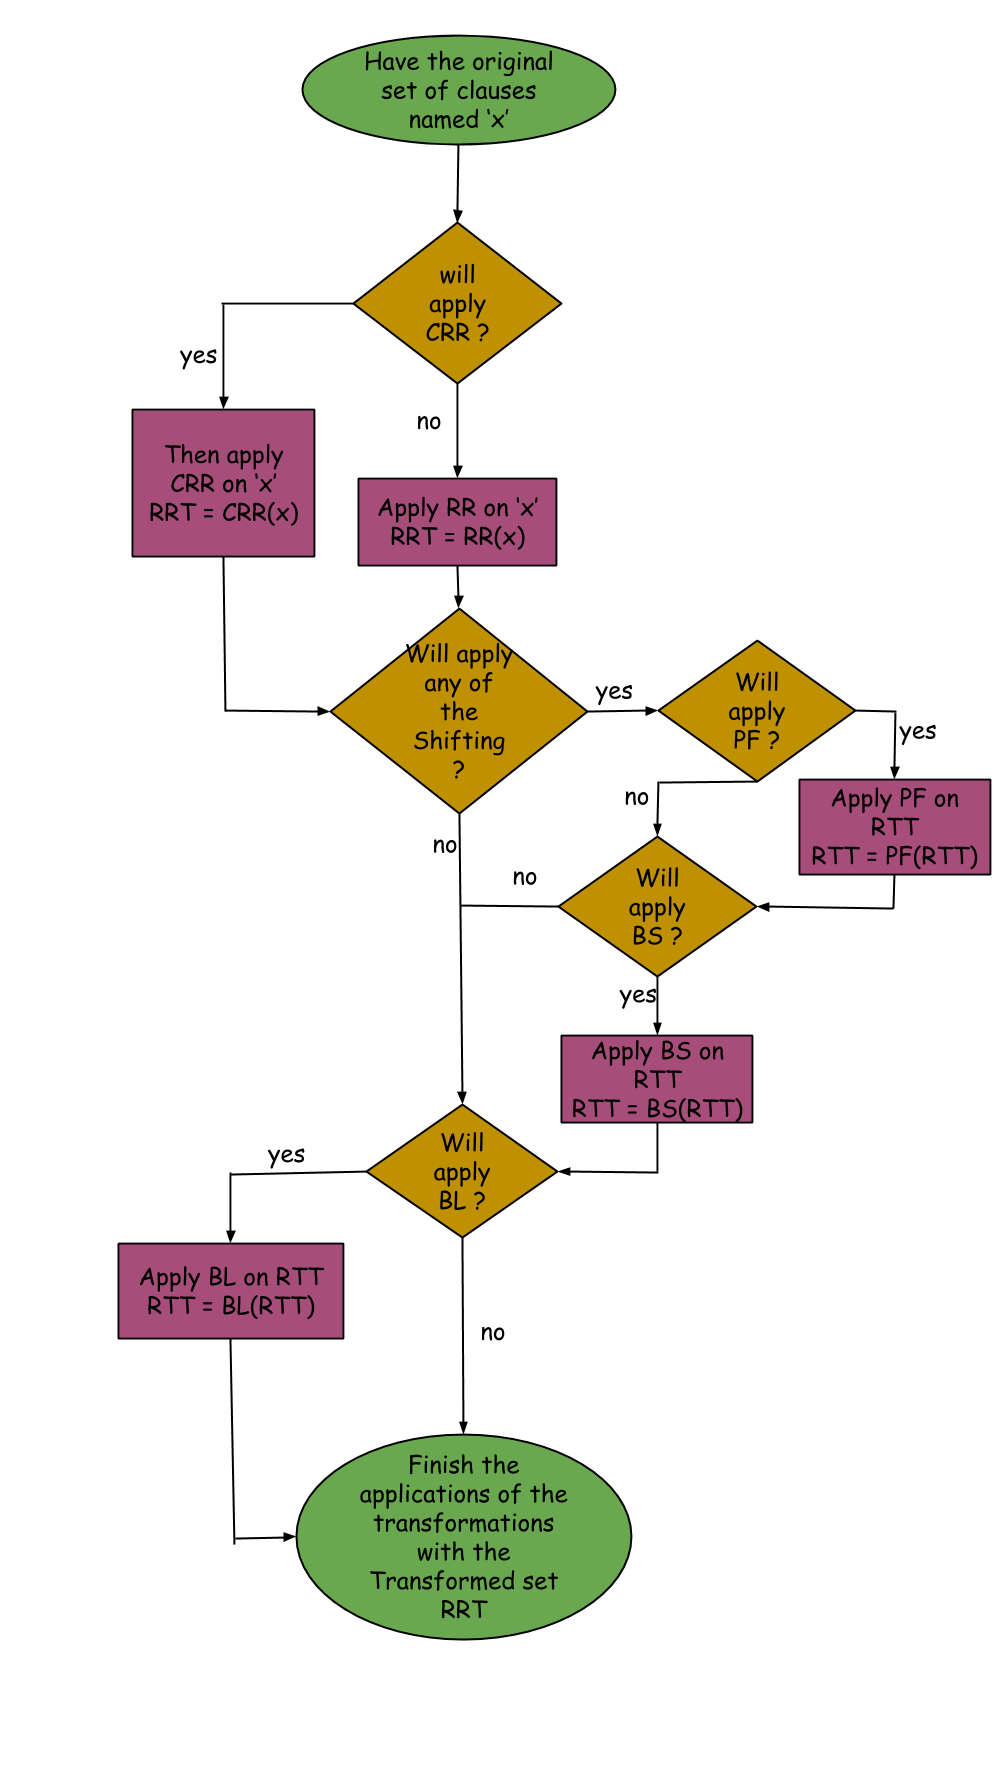
\includegraphics{pictures/Original_transformations_flow.png}}
 			\caption{Flow of the original transformations}\label{fig:original_transformations_flow}
		\end{figure}
	\subsection{Simplified transformations}\label{sub:c3s1s2}

This part is concerned about discussing the simplifications that were added to the original transformations highlighted in \ref{sub:c3s1s1}.
\\
Keeping in mind the definition of \ac{epr} as mentioned here in \ref{sub:c2s1s4}.
\\
So the following were made to each of the procedures:
\\
1- Every step that only deals with proper function symbols is removed since they are not existing in \ac{epr}.
\\
2- Any step or procedure that was introduced because of the existence of problems because of proper function symbols were removed as well. Ex.: pf, sh, and bl.
\\
\\
Therefore the resultant simplified procedures are the following:
\\
For crr:
\\
(0) Initialization. Initially, let crr(M) := M.
\\
(1) Add a constant. Let dom be a “fresh” unary predicate symbol not in ΣP , and let c
be some constant. Extend crr(M) by the clause dom(c) ← . (The constant c can
be “fresh” or belong to Σ f .)
\\
(2) Range-restriction. For each clause H ← B in crr(M), let {x1 , . . . , xk } be the set of
variables occurring in H but not in B . Replace H ← B by the clause
H ← B ∧ dom(x1 ) ∧ · · · ∧ dom(xk ).
\\
\\
For rr:
\\
(0) Initialization. Initially, let rr(M) := M.
\\
(1) Add a constant. Same as Step (1) in the definition of crr.
\\
(2) Domain elements from clause bodies. For each clause H ← B in M and each atom
P(t1 , . . . ,tn ) from B , let P(s1 , . . . , sn ) be the term abstraction of P(t1 , . . . ,tn ) and let α be the corresponding abstraction substitution. Extend rr(M) by the set
{dom(xi )α ← P(s1 , . . . , sn ) | 1 ≤ i ≤ n and xi → ti ∈ α}.
\\
(3) Range-restriction. Same as Step (2) in the definition of crr.
\\
(4) Domain elements from ΣP . For each n-ary P in Σ p , extend rr(M) by the set
{dom(xi ) ← P(x1 , . . . , xn ) | i ≤ i ≤ n}.


  
	
	\section{Model Construction}\label{sec:c3s2}
\paragraph{}
A Model Construction Technique had to be applied to the saturated set of clauses. This saturated set came from applying the normal prover to the transformed set of clauses. In our case the simplified version of the range restricting transformations is the one implemented. Here in this section we will cover the following points:

	\begin{itemize}
		\item What is the Model Construction Technique used
		\item How does it work
		\item Discussion on the Output
	\end{itemize}
	
	
	\subsubsection{What is the used technique for Model Construction}
		\paragraph{}
		The Model Construction Technique used is specific for resolution based theorem provers, and it is the ground positive case of Bachmair and Ganzinger Model Construction Technique that was devised here in \cite{BGMC}. This technique originated from the proof of Bachmair and Ganzinger that their resolution based theorem proving technique is complete. That proof will be found in \cite{BAGA01}.
		 %TODO check this info later ??
		
		
	\subsubsection{How does Bachmair and Ganzinger Model Construction Technique works}
		\paragraph{}		
		The chosen and implemented Bachmair and Ganzinger Model Construction Technique works for a saturated (counter) satisfiable set of positive ground set of clauses. That has been generated using an ordered resolution system with simplification. 
		
		\paragraph{}
		This Technique needs a term ordering that has been lifted to literals then lifted to clauses. That clause ordering should be total on ground clauses, and it should be the same one used in the saturation procedure. For an explanation of term orderings, you can refer to \cite{BAGA94}. And for specific discussion on the implemented orderings in the theorem prover E refer to \cite{E13}. 
		
		\paragraph{}
		The algorithm works as follows:
			
			\begin{enumerate}
				\item sort the positive ground clauses using the ordering in an ascending order
				\item sort the literals in each clause to define the maximal literal in descending order in terms of the ordering
				\item for each of the clauses starting from the smaller in terms of the ordering if not already true by the chosen true literals, then add the its maximal literal to the set of the chosen true literals 
			\end{enumerate}
		
		\paragraph{}
		A pseudo-code for the implemented version of the algorithm is given below:



%%%%%% commented old version of code %%%%%%

\begin{comment}
			\begin{minipage}{\textwidth}		
			\begin{lstlisting}[caption=Ground Positive Case for Bachmair and Ganzinger Model Construction,frame=single]
Input: clauses_set % saturated set of clauses
	, ordering % ordering used in the saturation
{	
	% model is the set of positive literals in the 
	% constructed model, at the beginning it is
	% an empty set of literals 
	model = {}			
				
	% this sorts the set of clauses ascendingly
	sort_clauses(clauses_set, ordering)  
	% it marks the maximal literal in each clause			
	mark_maximal_literals(clauses_set, ordering)
		
	for clause:clause_set do:
	{
	  % here it checks whether the current clause
	  % is true by the partial model we have or not
	  if not is_clause_true_by_model(clause, model) then:
	  {
		% if not true yet the it gets the marked
		% maximal literal and adds it to model											
		model = model + get_maximal_literal(clause)				
	  }
	  end_if
	}
	end_for						
}
Output: model
			\end{lstlisting}
			\end{minipage}		
\end{comment}

%			\begin{minipage}{\textwidth}		
			\begin{algorithm}[H]
			\caption{Ground Positive Case for Bachmair and Ganzinger Model Construction}
			\label{alg:bach_ganz_code}
				\begin{algorithmic}[1]
					\Procedure{extract\char`_model}{$clauses\char`_set, ordering$}
					
					\Comment {\parbox[t]{.7\linewidth}{$clauses\char`_set$ is the saturated set of clauses}}
				
					\Comment {\parbox[t]{.7\linewidth}{$ordering$ is the used ordering in the saturation}}
		

					\State let $model$ $\leftarrow$ $\lbrace \rbrace$

					\Comment {\parbox[t]{.7\linewidth} {$model$ is the set of positive literals in the constructed model at the beginning it is an empty set}} 
					

					\State $sort\char`_literals(clauses\char`_set, ordering)$	

					\Comment {\parbox[t]{.7\linewidth}{$sort\char`_literals$ sorts the literals in each clause descendingly}}	
					

					\State $sort\char`_clauses(clauses\char`_set, ordering)$

					\Comment {\parbox[t]{.7\linewidth}{$sort\char`_clauses$ sorts the clauses ascendingly in the clause set}}
					
					\For{each clause $c$ \Pisymbol{psy}{206} $clauses\char`_set$ }

						\If{$is\char`_true\char`_by\char`_model(c) \not= true$}
						
						\Comment {\parbox[t]{.7\linewidth}{$is\char`_true\char`_by\char`_model$ checks whether the current clause is true by the partial model we have or not}}
						

						\State set $model$ $\leftarrow$ $model$ + $get\char`_maximal\char`_literal(c)$
						
						\Comment {\parbox[t]{.7\linewidth}{$get\char`_maximal\char`_literal$ if not true yet the it gets the maximal literal, which is the first one since it is sorted, and adds it to model}}

						\EndIf

					\EndFor
					
					
					\State \textbf{return} $model$

					\EndProcedure
	\begin{comment}
Input: clauses_set % saturated set of clauses
	, ordering % ordering used in the saturation
{	
	% model is the set of positive literals in the 
	% constructed model, at the beginning it is
	% an empty set of literals 
	model = {}			
				
	% this sorts the set of clauses ascendingly
	sort_clauses(clauses_set, ordering)  
	% it marks the maximal literal in each clause			\usepackage[T1]{fontenc}
	mark_maximal_literals(clauses_set, ordering)
		
	for clause:clause_set do:
	{
	  % here it checks whether the current clause
	  % is true by the partial model we have or not
	  if not is_clause_true_by_model(clause, model) then:
	  {
		% if not true yet the it gets the marked
		% maximal literal and adds it to model											
		model = model + get_maximal_literal(clause)				
	  }
	  end_if
	}
	end_for						
}
Output: model
\end{comment}
				\end{algorithmic}
			\end{algorithm}
%			\end{minipage}	

		\paragraph{}
		In the implementation, We made a great use of the shared terms implemented in E. Since each term is only represented once in a term bank. So we added an attribute for the term structure representing whether it is evaluated to true or false. Comparison functions that takes the ordering into consideration were implemented. One is used for sorting the literals in a given clause. The other is for sorting the clauses in the clause set.		
		
		
		\paragraph{}
		An Example for applying the Bachmair and Ganzinger Model Construction Technique is given below:

			\begin{minipage}{\textwidth}
			\begin{lstlisting}[caption=Example for applying Bachmair and Ganzinger Model Construction Technique (SETUP),frame=single,mathescape]
	Let the unordered saturated set of clauses be:
	{
		$R(a, b) | Q(b)$,
		$P(a)$,
		$P(a) | Q(b)$,
		$R(b, b)$
	}
	
	Let the order of the present clauses:
	{
		P(a) < Q(b) < R(a, b) < R(b, b)
	}			

	% the left most literal in each of the
	% ordered clauses is the maximal
		\end{lstlisting}	
	
\begin{table}[H]
		\centering
		\begin{tabular}{||c | c | c | c||}
		\toprule		
		Order & Ordered Clause & Partial Model & Change in Model \\ [0.5ex] 
		\midrule
 		(1) & P(a) 			& {} 				& P(a) \\ 
 		(2) & Q(b) $\vert$ P(a)  	& {P(a)} 			& --- \\
 		(3) & R(a, b) $\vert$ Q(b)	& {P(a)}		 		& R(a, b) \\
 		(4) & R(b, b) 		& {P(a), R(a, b)} 	& R(b, b) \\ [1ex]
		\bottomrule		
		\end{tabular}
		\caption{Applying Model Construction Technique}
		\label{table:app_model}
\end{table}

		
			\begin{lstlisting}[caption=Example for applying Bachmair and Ganzinger Model Construction Technique (OUTPUT),frame=single,mathescape]
	Then the explicit Model:
	{
		$P(a)$,
		$R(a, b)$,
		$R(b, b)$	
	}		
			\end{lstlisting}
			\end{minipage}
		
		
%Then the ordered clauses	 :  partialModel		  : change in the partial model
%	{
		% the left most literal in each clause is the maximal
%		(1) $P(a)$			 :	{}				  :		$P(a)$
%		(2) $Q(b) | P(a)$	 :	{$P(a)$}			  :		-----
%		(3) $R(a, b) | Q(b)$	 :	{$P(a)$}			  :		$R(a, b)$
%		(4) $R(b, b)$		 :	{$P(a), R(a, b)$	} :		$R(b, b)$
%	}
	

	\subsubsection{Discussion on the Output}
		\paragraph{}		
		The output of the Model Construction Technique is the final one. It gives back the positive literals in the constructed explicit model. An Example for the output is given below in \ref{list:model_example}.
		
		
			\begin{minipage}{\textwidth}
			\begin{lstlisting}[caption=Example for the returned Model,label={list:model_example},frame=single]
		dom(t).
		bird(t).
		fly(t).
			\end{lstlisting} 
			\end{minipage}						
				
		\paragraph{}
		Moreover, we augmented the output with a visual part. It prints out a dot graph representing the positive clauses linked with the positive literal, that belongs to the model, that makes them true or satisfiable in other words. Example of the returned dot graph will be listed in \ref{list:dot_graph}, and a rendered Figure for the same graph will be in \ref{fig:dot_graph}.
		
			\begin{minipage}{\textwidth}
			\begin{lstlisting}[caption=Example of returned dot graph,label={list:dot_graph},breaklines=true,frame=single]
digraph model {
 rankdir=LR;
 subgraph cluster_model {
  label="Model"; 
  0 [shape=ellipse,fillcolor=lightskyblue1,style=filled,label="fly(t)"]
  1 [shape=ellipse,fillcolor=lightskyblue1,style=filled,label="bird(t)"]
  2 [shape=ellipse,fillcolor=lightskyblue1,style=filled,label="dom(t)"]
 }
 subgraph cluster_clauses {
  label="Positive Ground Clauses"; 
  3 [shape=box,fillcolor=lightpink1,style=filled,label="cnf(i_0_3, plain, (fly(t)))."]
  3 -> 0
  4 [shape=box,fillcolor=lightpink1,style=filled,label="cnf(i_0_1, plain, (bird(t)))."]
  4 -> 1
  5 [shape=box,fillcolor=lightpink1,style=filled,label="cnf(i_0_2, plain, (dom(t)))."]
  5 -> 2
 }
}
			\end{lstlisting} 
			\end{minipage}						

						
			\begin{figure}[H]
				\centering
				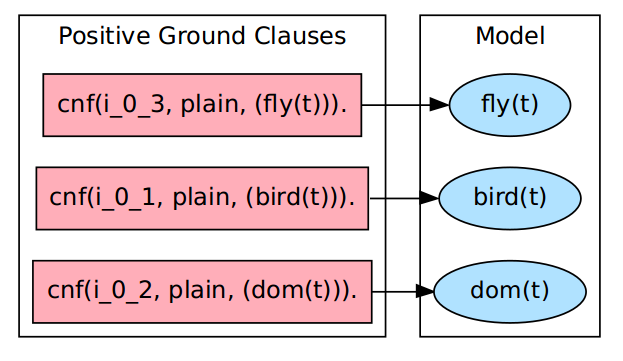
\includegraphics[scale=0.42]{pictures/dot_graph.png}
				\caption{Rendered dot graph of Model\label{fig:dot_graph}}
			\end{figure}
		
	\section{Code Flow}